\section{(2.29)}

The odd bound states involve a choice of the odd function in the $0<x<a$ region, which in this case is the sine, so our total wavefunction is

\begin{equation}
    \psi(x) = 
        \begin{alignedat}{1}
        \begin{cases}
            Fe^{-kx} \qquad & x>a, \\
            C\sin(\ell x)   & 0<x<a, \\
            -\psi(-x)       & x<0.
        \end{cases}
        \end{alignedat}
\end{equation}

Continuity of $\psi(x)$ at $x=a$ means that

\begin{equation*}
    Fe^{-ka} = C\sin(\ell a).
\end{equation*}

Continuity of $\dd\psi(x)/\ddx$ at $x=a$ means that

\begin{equation*}
    -kFe^{-ka} = \ell C\cos(\ell a).
\end{equation*}

Dividing the second by the first gives

\begin{equation*}
    -k = \ell\cot(\ell a) \quad \rightarrow \frac{ka}{\ell a} = -\cot(\ell a).
\end{equation*}

Using the definition $z = \ell a$ and $z_0 = \frac{a}{\hbar}\sqrt{2mV_0}$, as well as the fact from the book that $ka = \sqrt{z_0^2 - z^2}$, we arrive at a very similar (but not exact) transcendental equation for $z$:

\begin{equation}
    -\cot(z) = \sqrt{\br{\frac{z_0}{z}}^2 - 1}.\label{eq:Prblm3-TranscendentalEQ}
\end{equation}


\begin{figure}[ht]
    \centering
    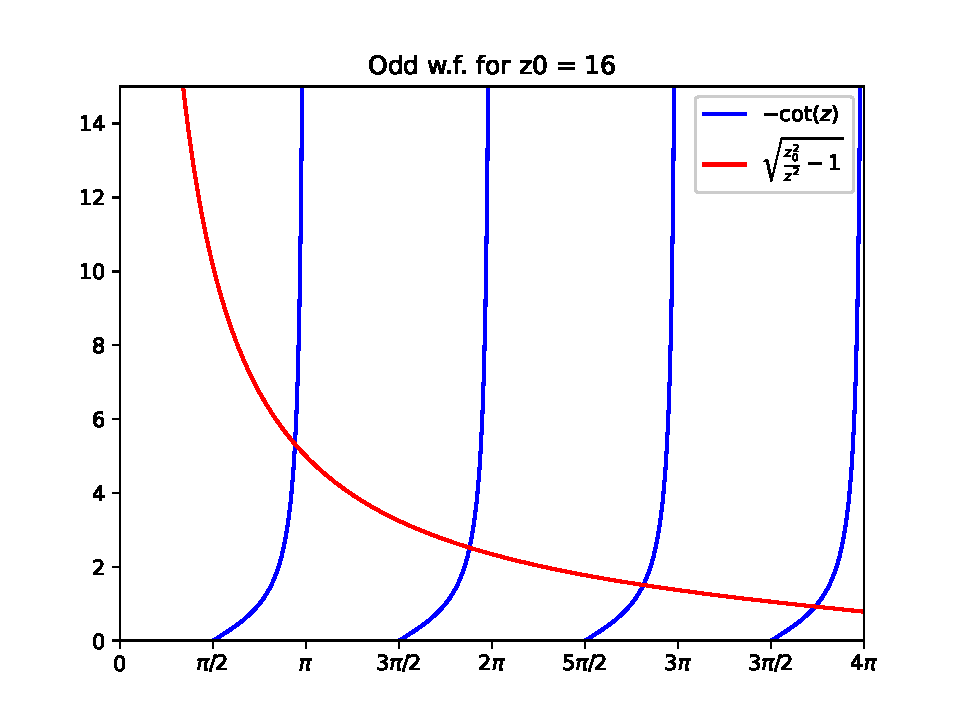
\includegraphics[width=0.4\linewidth]{./res/Prblm3_1.pdf}
    \hspace*{3mm}
    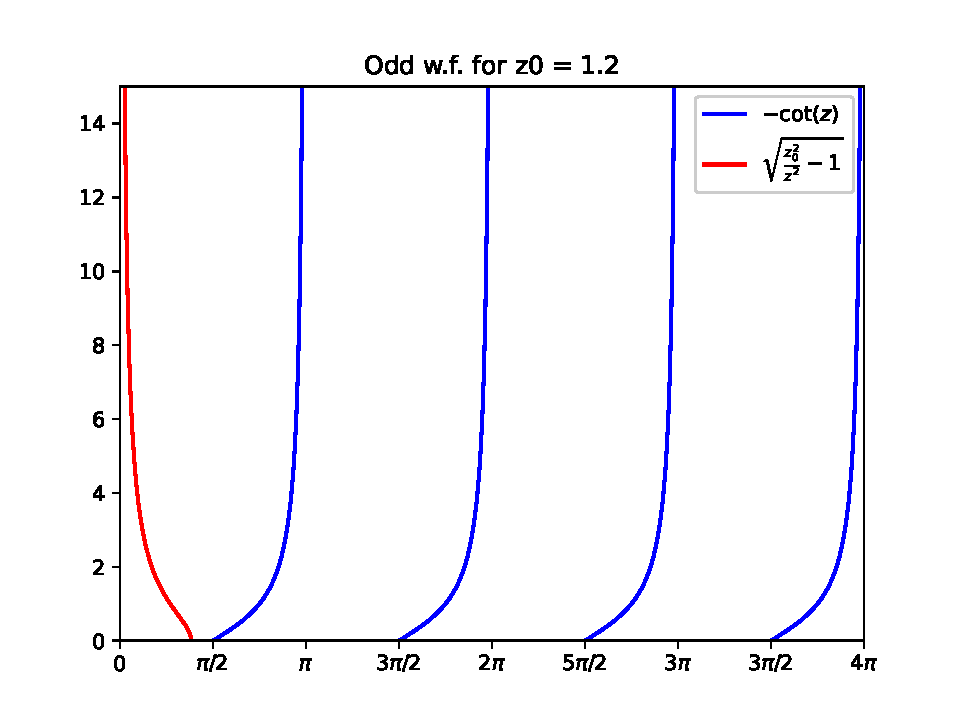
\includegraphics[width=0.4\linewidth]{./res/Prblm3_2.pdf}
    \caption{Plots of both sides of the transcendental equation in Equation~\eqref{eq:Prblm3-TranscendentalEQ} for $z_0 = 16$ (left) and $z_0 = 1.2$ (right).}
    \label{fig:Prblm3-TranscendentalPlots}
\end{figure}

In Figure~\ref{fig:Prblm3-TranscendentalPlots}, I plotted the left and right-hand sides of Equation~\eqref{eq:Prblm3-TranscendentalEQ}. On the left I set $z_0=16$, in which we can see a similar looking plot for that of the even solutions, where we have a number of intersections. However, in the right plot, I let $z_0$ go way down to 1.2, where we can see that there are actually no intersections, meaning that for some suitably small cutoff value $z_0$, there are no longer any bound states. This corresponds to a particularly shallow or small well.

In the other limiting case with $z_0 \rightarrow \infty$ (a wide, deeper well), we get a similar limiting case to before where the intersections occur at integer multiples of $\pi$. This time, though, they occur at the even multiples, which complement the odd multiples from the even wavefunction.